\chapter{Appendix}
\label{chap:appendix}

In section \ref{sec:optimizer-comparison}, I presented a characterization of
the \texttt{Crotosolve} loss curve in comparison to other optimizers used in
quantum machine learning.
While the analysis was illustrated with a single example, this section contains
the loss curves of further PQCs.
The circuit ids referenced in the captions refer to the circuit template numbers
from \cite{sim_expressibility_2019}.
All tests use circuits with four qubits and three template layers.
The source code for the dataset generation and visualization is available with
the \texttt{Crotosolve} implementation \cite{crotosolve}.

\begin{figure}
    \centering
    \subfloat[subcaption]{
        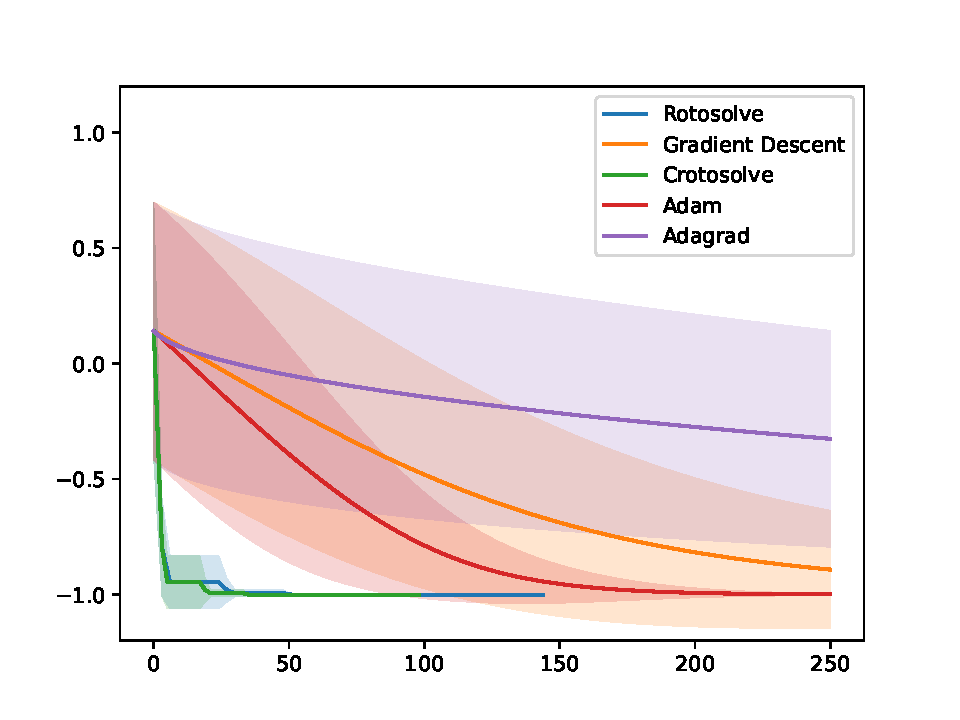
\includegraphics[width=0.5\textwidth]{loss-curve_sim01_4x3.pdf}
    }
    \subfloat[subcaption]{
        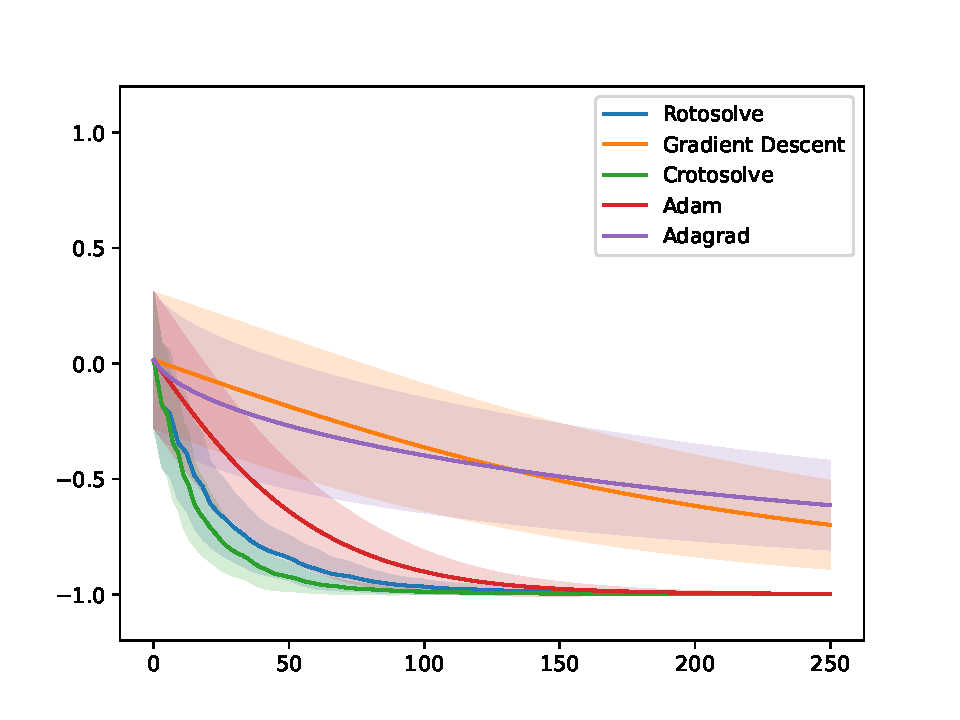
\includegraphics[width=0.5\textwidth]{loss-curve_sim02_4x3.pdf}
    }
    \caption{Caption goes here}
\end{figure}
\begin{figure}\ContinuedFloat
    \centering
    \subfloat[subcaption]{
        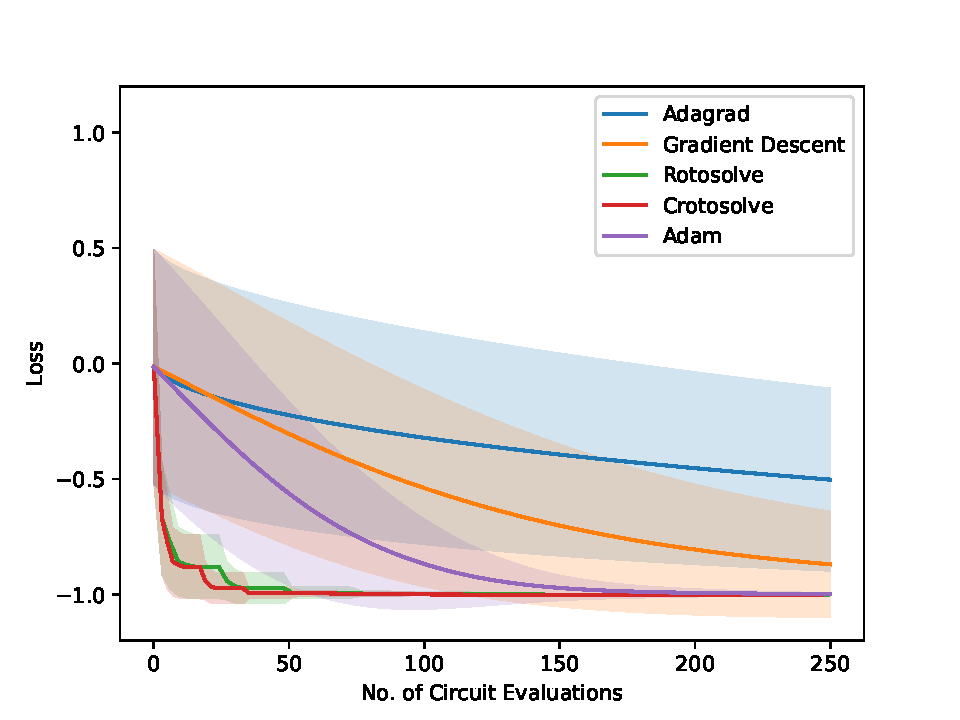
\includegraphics[width=0.5\textwidth]{loss-curve_sim03_4x3.pdf}
    }
    \subfloat[subcaption]{
        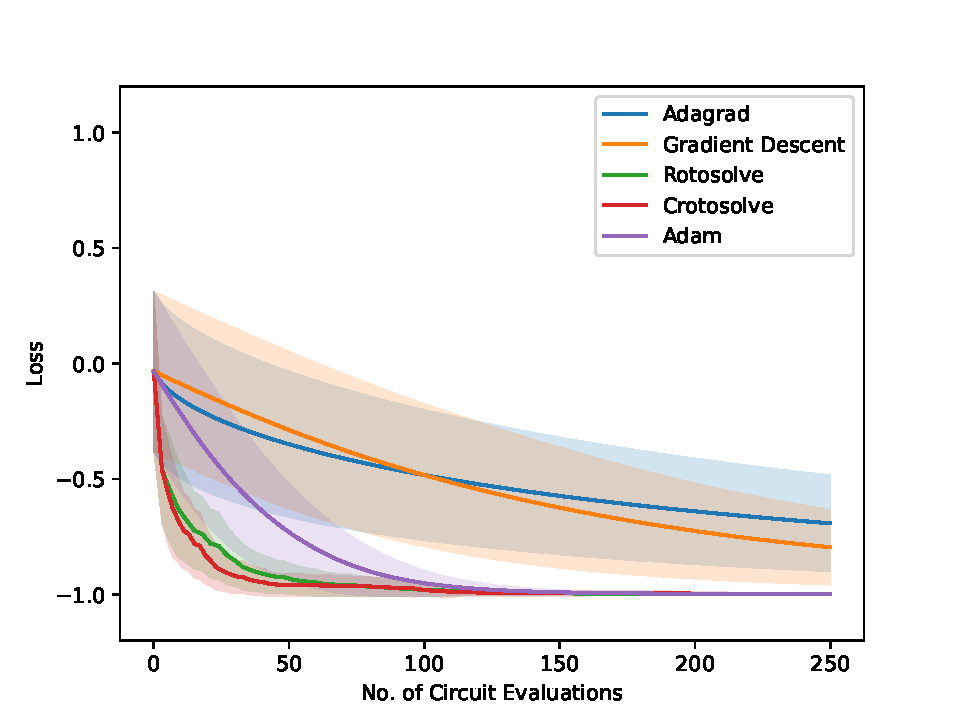
\includegraphics[width=0.5\textwidth]{loss-curve_sim04_4x3.pdf}
    }
    \hspace{0mm}
    \subfloat[subcaption]{
        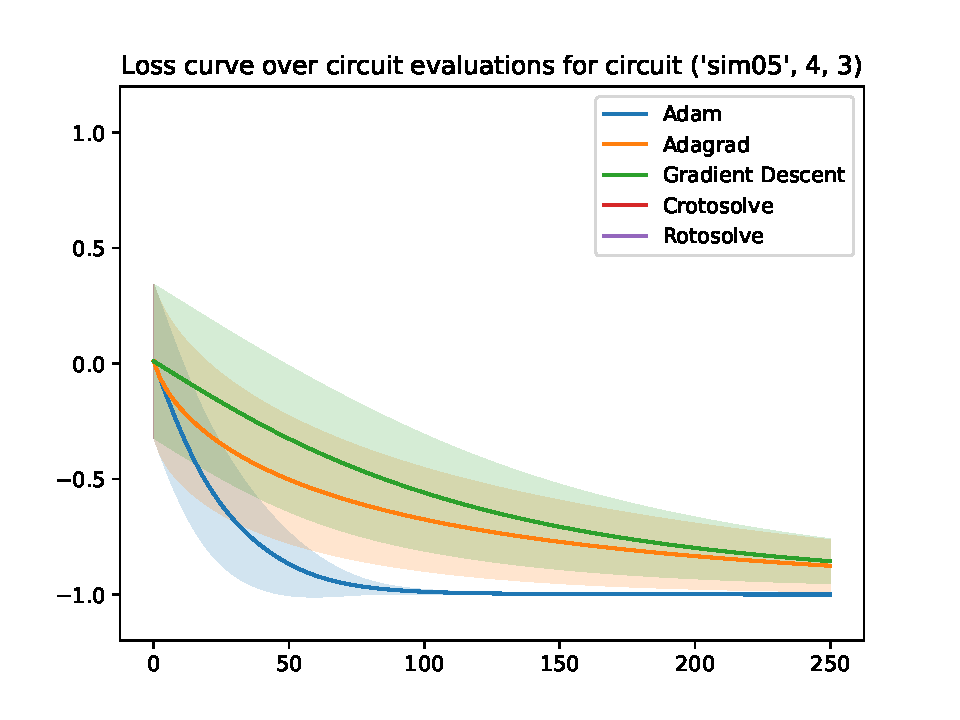
\includegraphics[width=0.5\textwidth]{loss-curve_sim05_4x3.pdf}
    }
    \subfloat[subcaption]{
        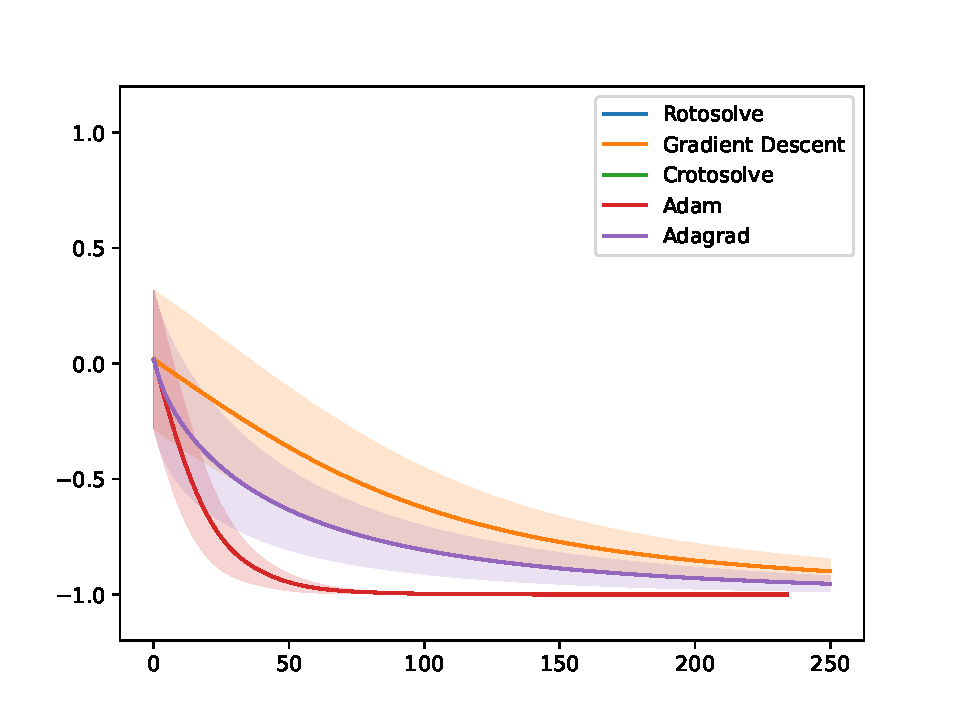
\includegraphics[width=0.5\textwidth]{loss-curve_sim06_4x3.pdf}
    }
    \hspace{0mm}
    \subfloat[subcaption]{
        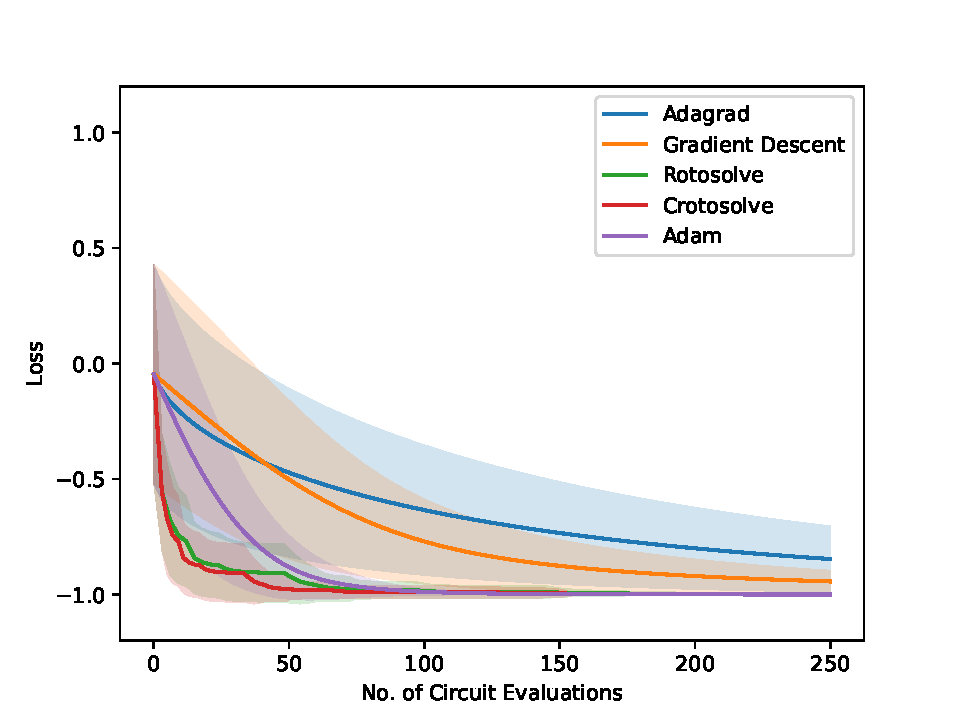
\includegraphics[width=0.5\textwidth]{loss-curve_sim07_4x3.pdf}
    }
    \subfloat[subcaption]{
        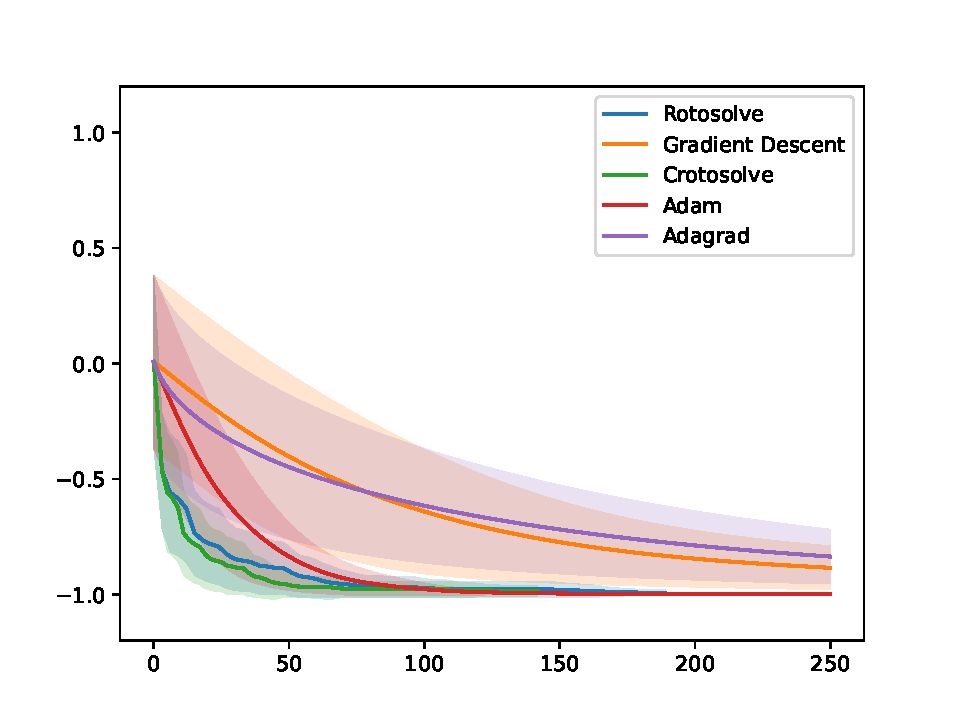
\includegraphics[width=0.5\textwidth]{loss-curve_sim08_4x3.pdf}
    }
    \caption{Caption goes here}
\end{figure}
\begin{figure}\ContinuedFloat
    \centering
    \subfloat[subcaption]{
        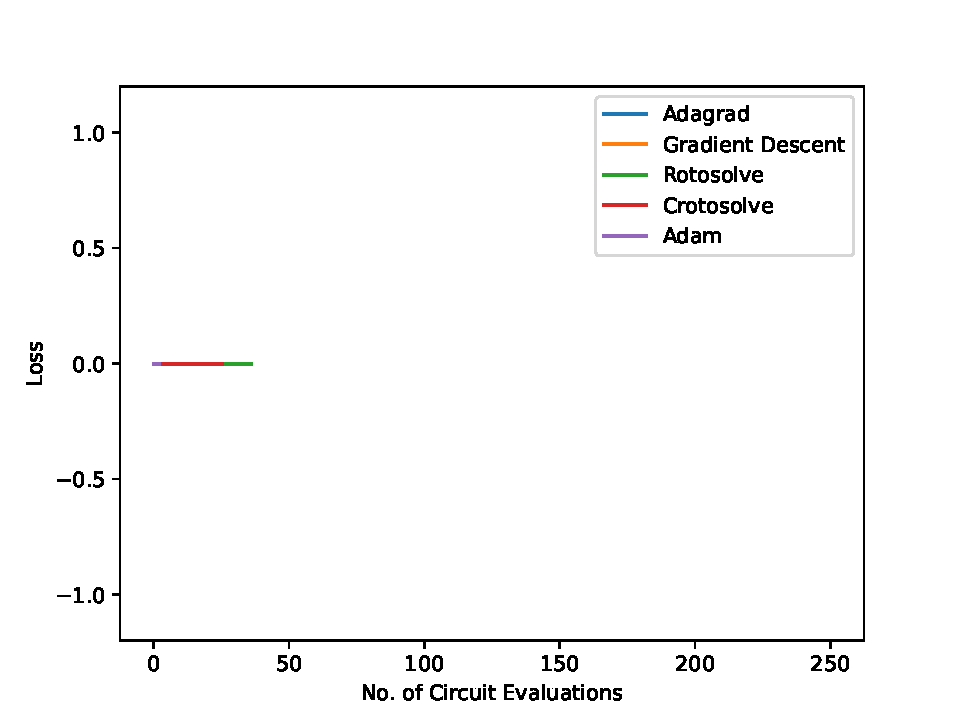
\includegraphics[width=0.5\textwidth]{loss-curve_sim09_4x3.pdf}
    }
    \subfloat[subcaption]{
        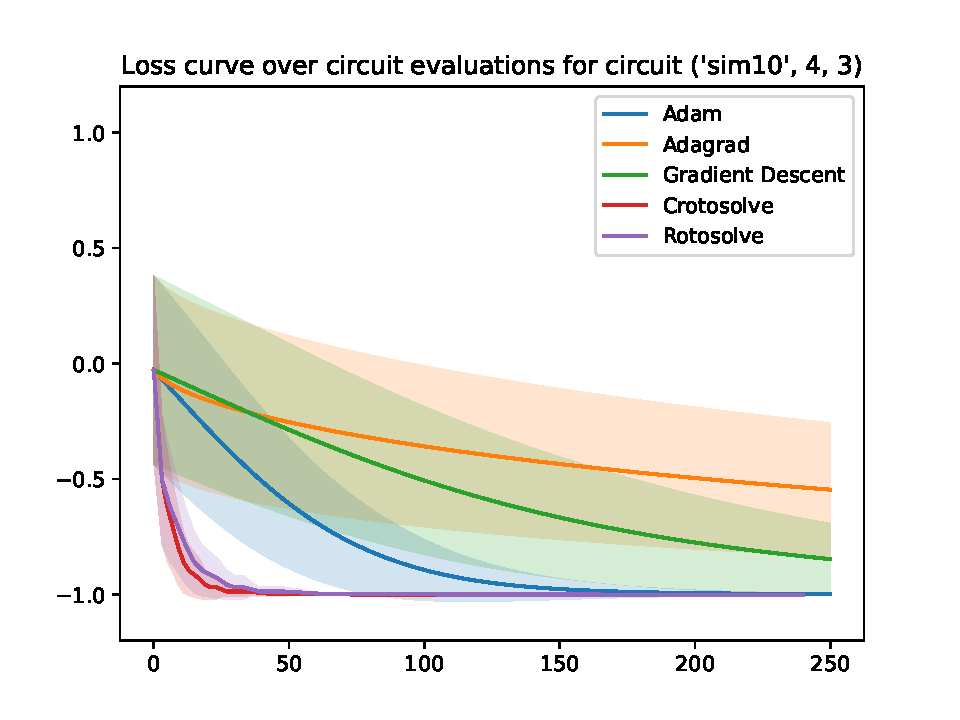
\includegraphics[width=0.5\textwidth]{loss-curve_sim10_4x3.pdf}
    }
    \hspace{0mm}
    \subfloat[subcaption]{
        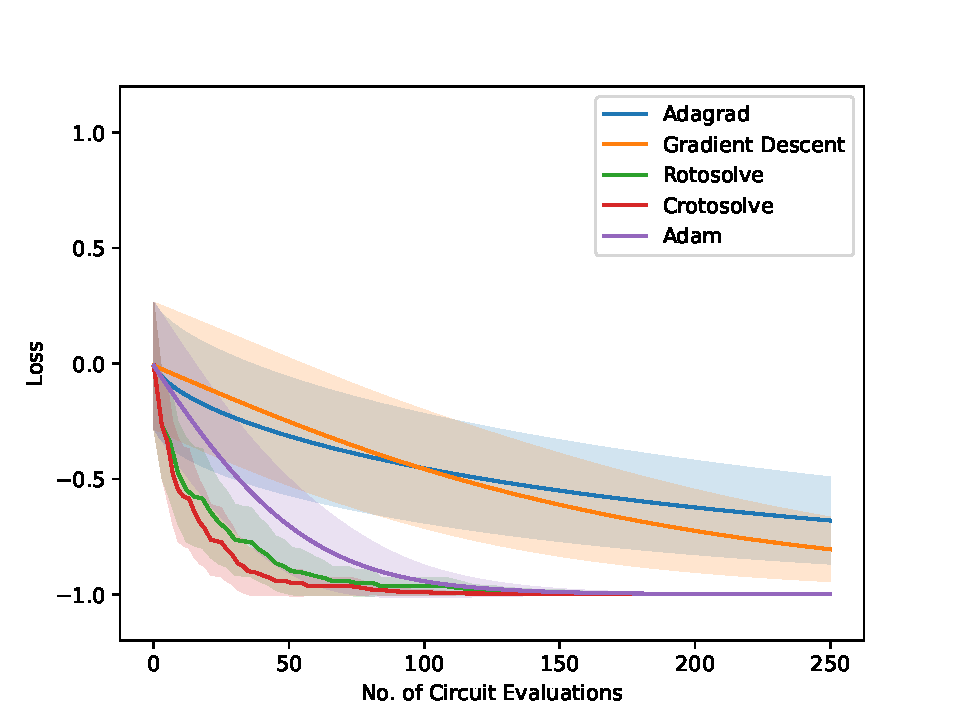
\includegraphics[width=0.5\textwidth]{loss-curve_sim11_4x3.pdf}
    }
    \subfloat[subcaption]{
        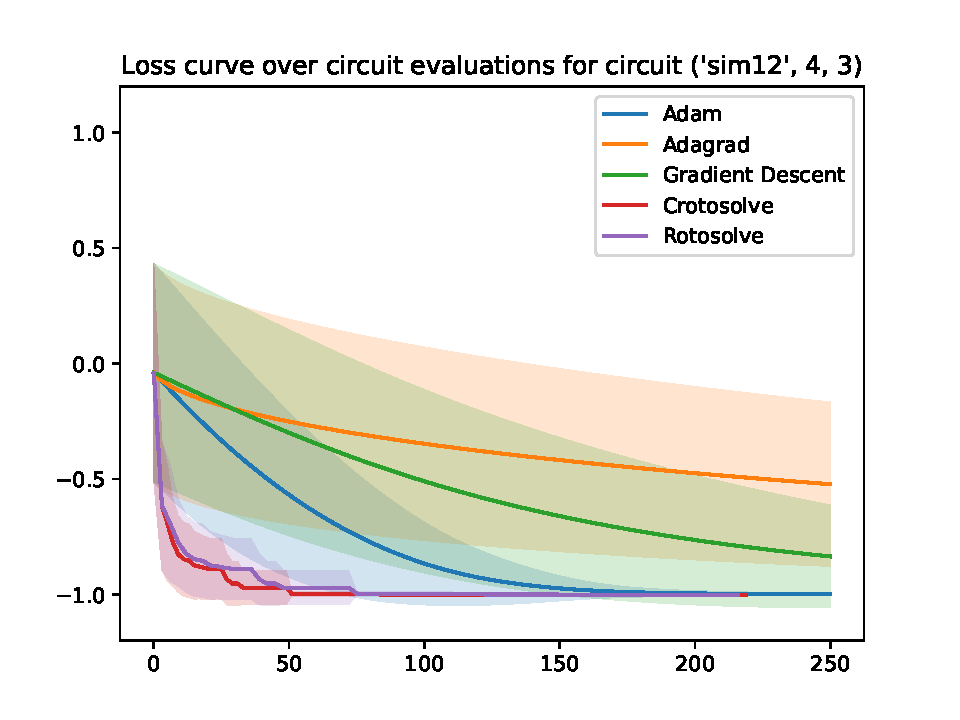
\includegraphics[width=0.5\textwidth]{loss-curve_sim12_4x3.pdf}
    }
    \hspace{0mm}
    \subfloat[subcaption]{
        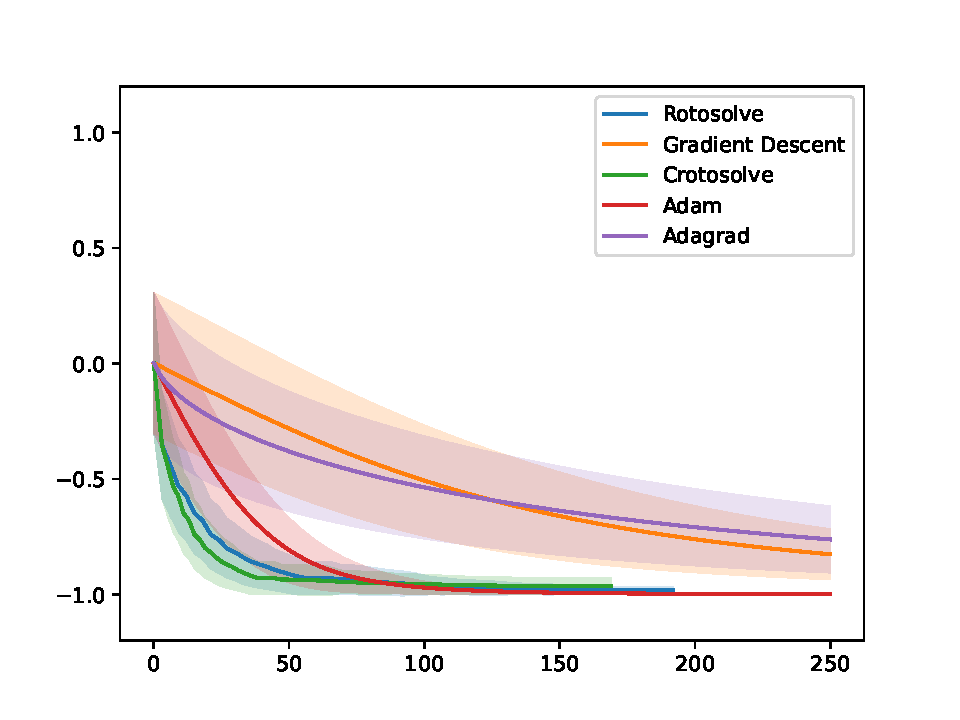
\includegraphics[width=0.5\textwidth]{loss-curve_sim13_4x3.pdf}
    }
    \subfloat[subcaption]{
        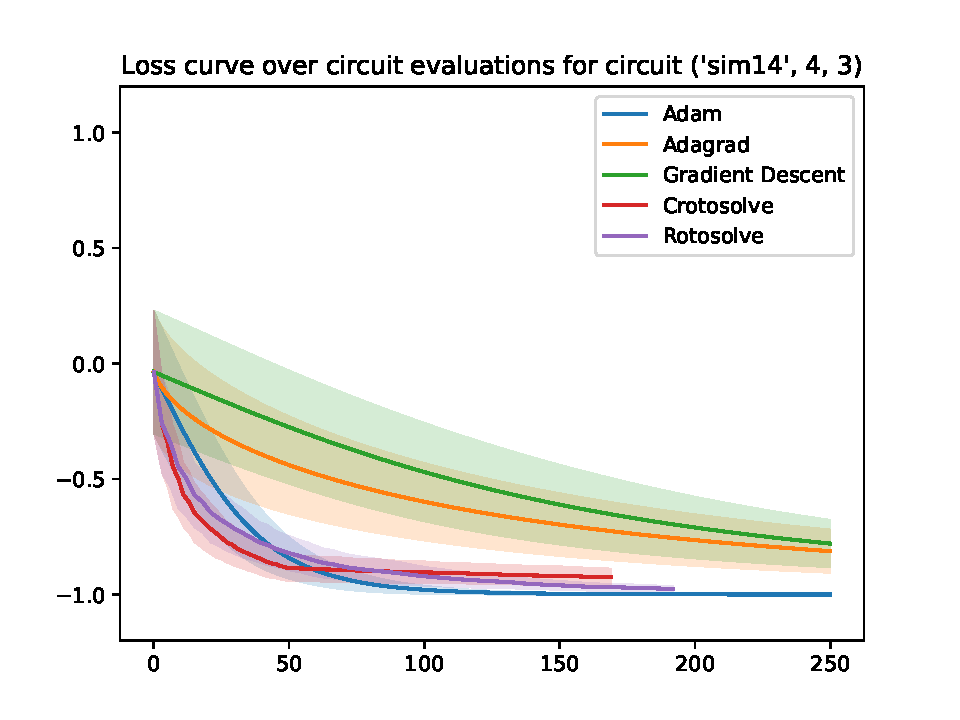
\includegraphics[width=0.5\textwidth]{loss-curve_sim14_4x3.pdf}
    }
    \caption{Caption goes here}
\end{figure}
\begin{figure}\ContinuedFloat
    \centering
    \subfloat[subcaption]{
        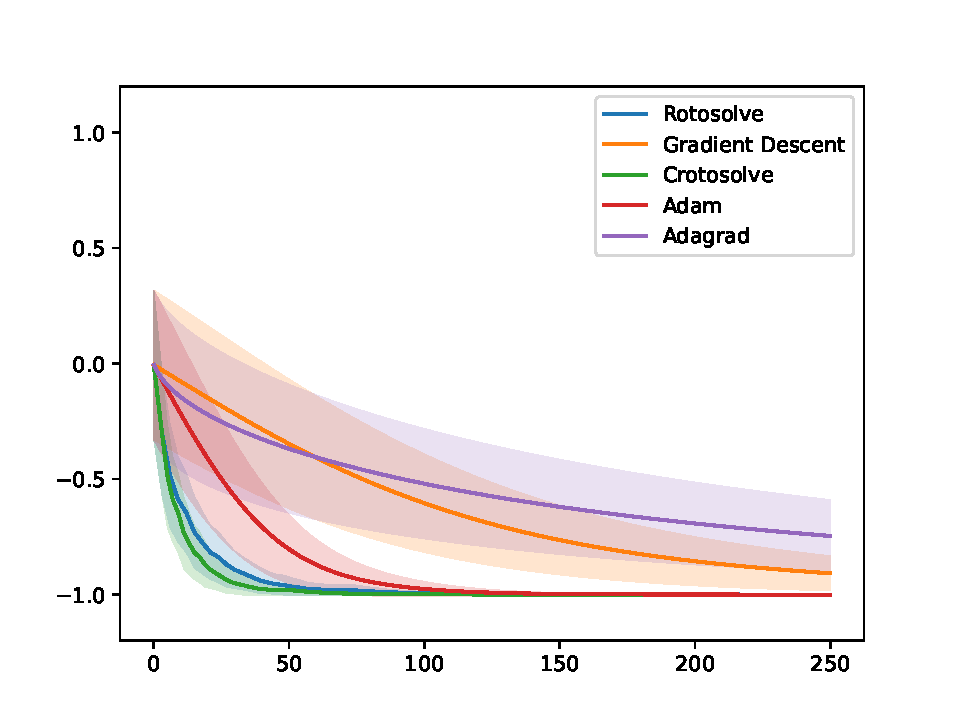
\includegraphics[width=0.5\textwidth]{loss-curve_sim15_4x3.pdf}
    }
    \subfloat[subcaption]{
        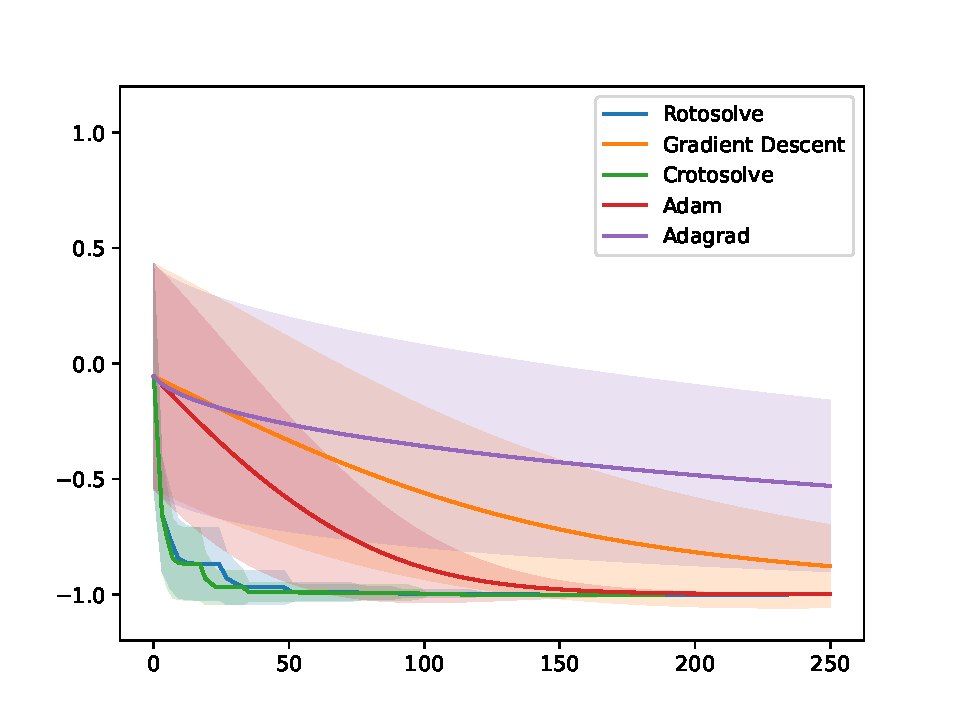
\includegraphics[width=0.5\textwidth]{loss-curve_sim16_4x3.pdf}
    }
    \hspace{0mm}
    \subfloat[subcaption]{
        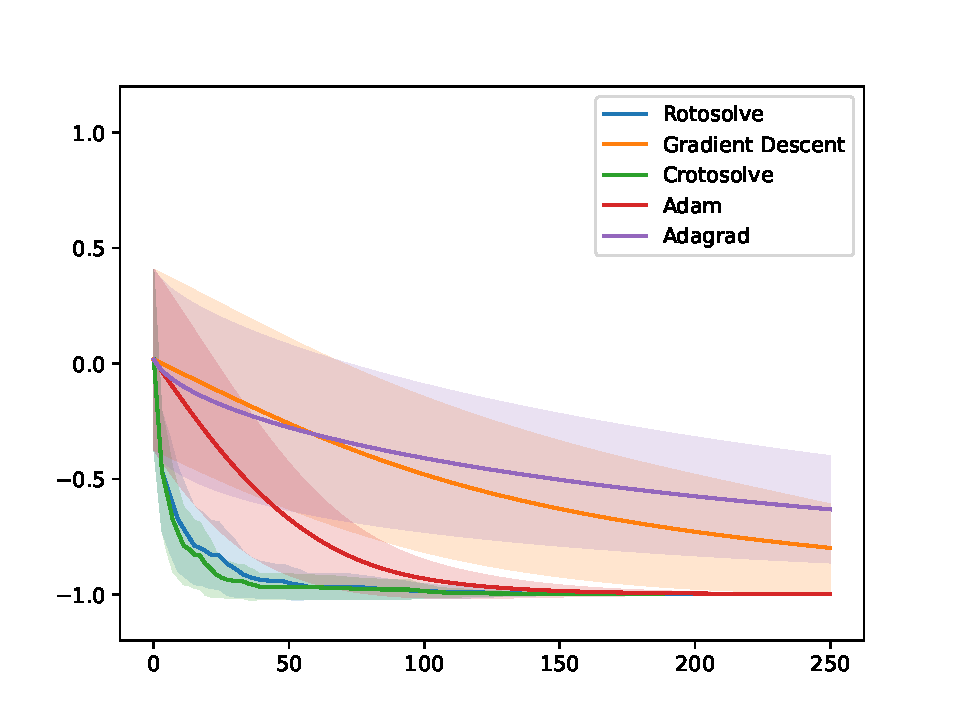
\includegraphics[width=0.5\textwidth]{loss-curve_sim17_4x3.pdf}
    }
    \subfloat[subcaption]{
        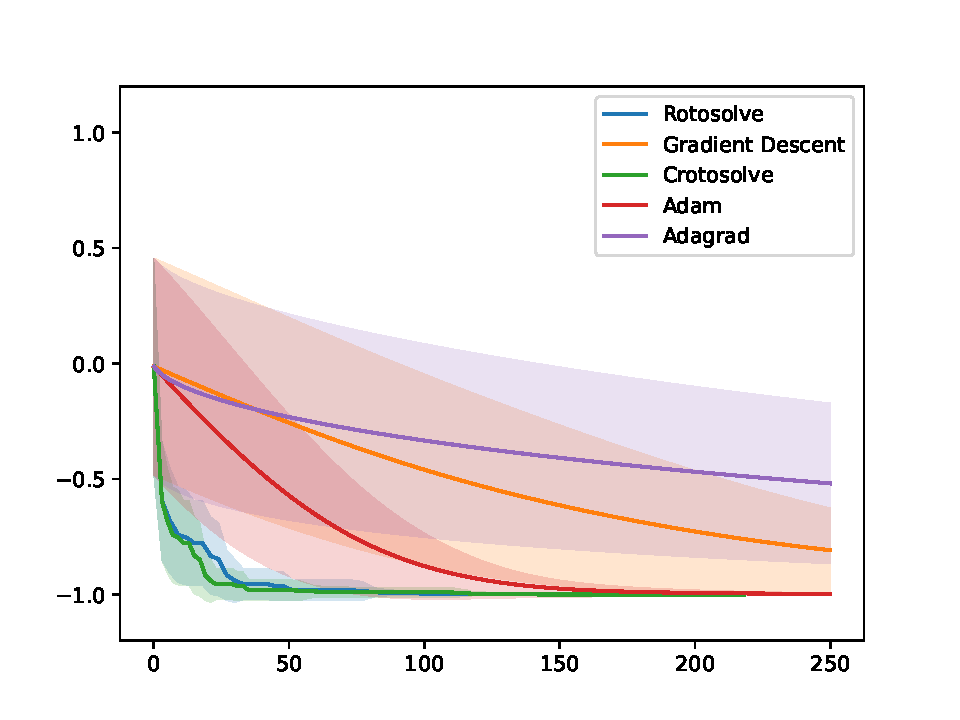
\includegraphics[width=0.5\textwidth]{loss-curve_sim18_4x3.pdf}
    }
    \hspace{0mm}
    \subfloat[subcaption]{
        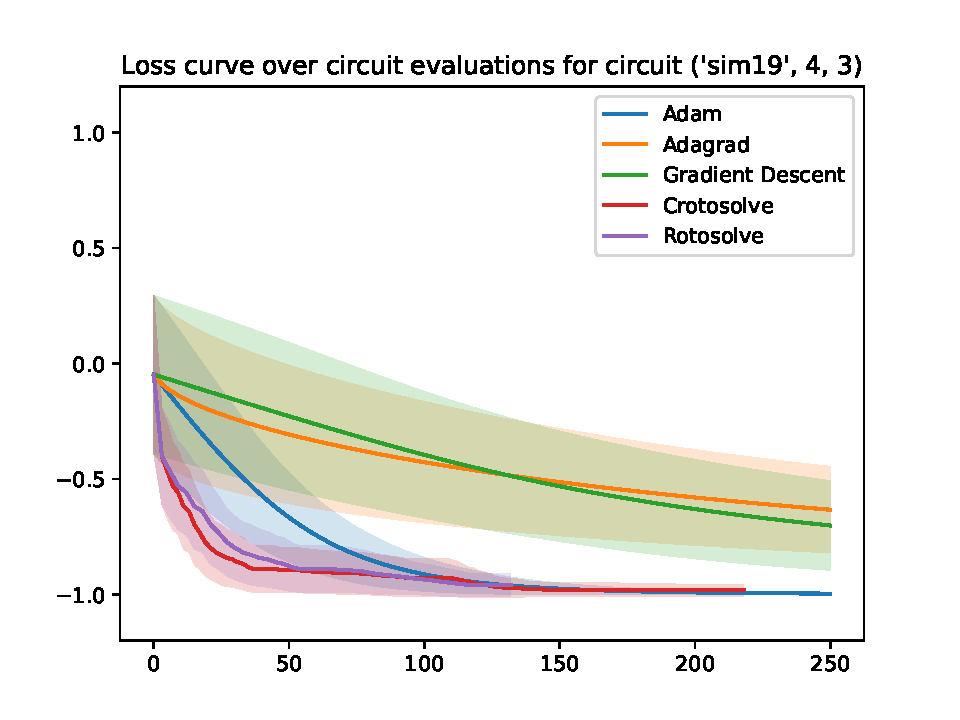
\includegraphics[width=0.5\textwidth]{loss-curve_sim19_4x3.pdf}
    }
    \caption{Caption goes here}
\end{figure}